\documentclass[MAS331_Note.tex]{subfiles}

\begin{document}
\chapter{Countability and Separation Axioms}
\section{The Countability Axioms}

\dfn{First Countability Axiom}{
    A topological space $X$ is said to have a \textit{countable basis at} $x$
    if there is a countable collection $\mcal B$ of neighborhoods of $x$ in $X$
    such that, for each neighborhood $U$ of $x$, there exists $B \in \mcal B$
    with $B \subseteq U$. A space that has a countable basis at each point is
    said to satisfy the \textit{first countability axiom}, or to be
    \textit{first-countable}.
}

\nt{
    This definition was already given in \Cref{def:1stCt}.
    Recall the lemmas \Cref{lem:seqLemma} and \Cref{lem:seqConvIffImgConv}.
}

\dfn{Second Countability Axiom}{
    If a topological space $X$ has a countable basis for its topology, then
    $X$ is said to satisfy the \textit{second countability axiom}, or to be
    \textit{second-countable}.
}

\exmp{}{
    $\RR[J]$ endowed with the product topology with a countable set $J$ is
    second-countable;
    \[
        \mcal S \triangleq \bigcup_{\alpha \in J} \big\{\, \pi_{\alpha}\inv
        \big((a, b)\big) \:\big|\: a, b \in \QQ \text{ and } a<b \big\}
    \]
    is a countable subbasis for $\RR[J]$, which induces a countable basis for
    $\RR[J]$.
}

\nt{
    If a topological space $X$ is second-countable with a countable basis
    $\mcal B= \{B_n\}_{n \in \ZZ_+}$ and a subspace $A \subseteq X$ with the
    discrete topology. Then, $A$ must be countable.

    Otherwise, for each $a \in A$, there exists $B_a \in \mcal B$ such that
    $B_a \cap A = \{a\}$. This induces an injection $A \hookrightarrow \mcal B$.
    Hence, $A$ is countable.
}

\exmp[RUnifNot2ndCt]{Uniform Topology and Countability Axioms}{
    In the uniform topology, $\RR[\omega]$ is first-countable by
    \Cref{exmp:metIs1stCt}. Let $\mcal B$ be a basis of $\RR[\omega]$. Let
    \[
        A \triangleq \big\{\,(x_i)_{i \in \ZZ_+} \in \RR[\omega] \:\big|\:
        \forall i \in \ZZ_+,\: x_i \in \{\,0, 1\,\}\,\big\}\text{.}
    \]
    Then, $A$ has the discrete topology but $A$ is uncountable. Therefore,
    $\RR[\omega]$ with the uniform topology is not second-countable.
}

\thm[subspCt]{}{
    Let $X$ be a topological space and $A$ be a subspace of $X$.
    \begin{itemize}[nolistsep]
        \ii If $X$ is first-countable, then $A$ is first-countable.
        \ii If $X$ is second-countable, then $A$ is second-countable.
    \end{itemize}
}
\pf{Proof}{
    \hfill
    \begin{itemize}[nolistsep]
        \ii Let $a \in A$. Let $\mcal B$ be a countable basis of $X$ at $a$.
            Then, $\{\,B \cap A \mid B \in \mcal B\,\}$ is a countable basis
            for the subspace $A$ at $a$. \checkmark
        \ii Let $\mcal B$ be a countable basis of $X$. Then, $\{\,B \cap A
            \mid B \in \mcal B\,\}$ is a countable basis for the subspace $A$.
            \checkmark
    \end{itemize}
}

\thm[prodCt]{}{
    Let $\{X_\alpha\}_{\alpha \in J}$ be a countable family of topological
    spaces.
    \begin{itemize}[nolistsep]
        \ii If each $X_i$ is first-countable, then $\prod_{\alpha \in J}
            X_\alpha$ in the product topology is first-countable.
        \ii If each $X_i$ is second-countable, then $\prod_{\alpha \in J}
            X_\alpha$ in the product topology is second-countable.
    \end{itemize}
}
\pf{Proof}{
    \hfill
    \begin{itemize}[nolistsep]
        \ii Let $(x_{\alpha})_{\alpha \in J} \in \prod_{\alpha \in J} X_\alpha$.
            Then, for each $\alpha \in J$, there exists a countable basis
            $\mcal B_\alpha$ of $X_\alpha$ at $x_\alpha$.
            Then, $\big\{\, \prod_{\alpha \in J} B_\alpha \:\big|\:
            \forall \alpha \in J,\: B_\alpha \in \mcal B_\alpha\,\big\}$ is a
            countable basis at $(x_\alpha)_{\alpha \in J}$.
        \ii For each $\alpha \in J$, there exists a countable basis $\mcal
            B_\alpha$ of $X_\alpha$. Then, $\big\{\,\prod_{\alpha \in J}
            B_\alpha \:\big|\: \forall \alpha \in J,\: B_\alpha \in \mcal
            B_\alpha\,\big\}$ is a countable basis of $\prod_{\alpha \in J}
            X_\alpha$.
    \end{itemize}
}

\dfn{Lindelöf Space}{
    A topological space $X$ is called a \textit{Lindelöf space} if, for every
    open covering of $X$, there is a countable subcovering.
}

\dfn{Dense Subset}{
    A subset $A$ of a topological space $X$ is said to be \textit{dense} in $X$
    if $\cl A = X$.
}

\dfn{Separable Space}{
    A topological space $X$ is said to be \textit{separable} if there is a
    countable dense subset of $X$.
}

\nt{
    Obvious facts:
    \begin{itemize}[nolistsep]
        \ii Every compact space is a Lindelöf space.
        \ii The box and product topologies on an finite product of separable
            spaces is separable.
            (\Cref{th:prodOfClosureIsClosureOfProd})
        \ii Every topology on a countable set is Lindelöf and separable.
   \end{itemize}
}

\thm[2ndCtThenLindAndSep]{}{
    Let $X$ be a second-countable space. Then,
    \begin{itemize}[nolistsep]
        \ii $X$ is a Lindelöf space.
        \ii $X$ is separable.
    \end{itemize}
}
\pf{Proof}{
    Let $\mcal B = \{B_n\}_{n \in \ZZ_+}$ be a countable basis for $X$.
    \begin{itemize}[nolistsep]
        \ii Let $\mcal A$ be an open covering of $X$. For each $n \in \ZZ_+$,
            there exists $A_n \in \mcal A$ such that $B_n \subseteq A_n$.
            Then, $\mcal A' \triangleq \{\,A_n \mid n \in \ZZ_+\,\}$ is a
            countable subcovering of $X$ as $\mcal B$ covers $X$. \checkmark
        \ii For each $n \in \ZZ_+$, choose $x_n \in B_n$. Let $D \triangleq
            \{\,x_n \mid n \in \ZZ_+\,\}$. Then, for all $x \in X$, every
            basis element that contains $x$ intersects $D$; $\cl D = X$
            by \Cref{th:inClosureIffNeighCapANonempty}. \checkmark
    \end{itemize}
}

\exmp[REllCt]{$\RR_\ell$ and Countability Axioms}{
    \begin{itemize}[nolistsep]
        \ii Given $x \in \RR_\ell$, $\{\,[x, x + 1/n) \mid n \in \ZZ_+\,\}$
            is a countable basis at $x$. $\RR_\ell$ is first-countable.
        \ii $\cl{\QQ} = \RR_\ell$. $\RR_\ell$ is separable.
        \ii Let $\mcal B$ be a basis for $\RR_\ell$. Choose, for each $x \in
            \RR_\ell$, an element $B_x \in \mcal B$ such that $x \in B_x
            \subseteq [x, x+1)$. If $x \neq y$, then $B_x \neq B_y$. Hence
            $x \mapsto B_x$ is an injection; $\mcal B$ is uncountable.
            Therefore, $\RR_\ell$ is not second-countable.
    \end{itemize}
    We now prove $\RR_\ell$ is Lindelöf. Thanks to \Cref{lem:topByBIsUnionsOfB},
    we only have to prove that, for any open covering $\mcal A$ of $\RR_\ell$
    by the basis elements, there is a countable subcovering.

    Let $\mcal A = \{\,[a_\alpha, b_\alpha) \mid \alpha \in J\,\}$ be an open
    covering of $\RR_\ell$. Let $C \triangleq \bigcup_{\alpha \in J} (a_\alpha,
    b_\alpha)$. We now claim that $\RR \setminus C$ is countable.
    Let $x \in \RR \setminus C$. Then $x = a_\beta$ for some $\beta \in J$.
    Choose $q_x \in \QQ$ such that $q_x \in (a_\beta, b_\beta)$.
    If $x, y \in \RR \setminus C$ and $x < y$, then $q_x < q_y$. Hence
    $x \mapsto q_x$ defines an injection $\RR \setminus C \hookrightarrow \QQ$.
    Therefore, $\RR \setminus C$ is countable.

    Now, let $\mcal A'$ be a countable subcollection of $\mcal A$ that covers
    $\RR \setminus C$. Now, note that $\{\,(a_\alpha, b_\alpha) \mid \alpha \in
    J\,\}$ is an open covering of $C$ as a subspace of $\RR$ (with the standard
    topology). Since $\RR$ is second-countable, there exists a finite
    subcollection $\{\,(a_{\alpha_1}, b_{\alpha_1}), \cdots, (a_{\alpha_n},
    b_{\alpha_n})\,\}$ covers $C$. Let $\mcal A'' \triangleq \{\,[a_{\alpha_1},
    b_{\alpha_1}), \cdots, [a_{\alpha_n}, b_{\alpha_n})\}$.
    Then, $\mcal A' \cup \mcal A''$ is a countble subcovering of $\RR_\ell$.
}

\exmp[sorgenfrey]{The Product of Two Lindelöf Spaces Need Not Be Lindelöf}{
    Although $\RR_\ell$ is Lindelöf, $\RR_\ell \times \RR_\ell$ is not.
    Consider the subspace $L \triangleq \{\,x \times (-x) \mid x \in
    \RR_\ell\}$. Then, $L$ has the discrete topology as $\big([x, x+1) \times
    [-x, -x+1)\big) \cap L = \{x \times (-x)\}$. Hence, $L$ is not Lindelöf;
    $\RR_\ell^2$ is not Lindelöf.
}

\exmp{A Subspace of a Lindelöf Space Need Not Be Lindelöf}{
    The ordered square $I_o^2$ is compact (\Cref{exmp:orderedSqIsCpt}) and thus
    is Lindelöf. However, the subspace $A = I \times (0, 1)$ is not Lindelöf
    as an open covering $\{\,\{x\} \times (0, 1) \mid x \in I\,\}$ does not
    allow a countable subcovering.
}

\nt{
    Here is the diagram that represents the relations between spaces.
    \begin{center}
    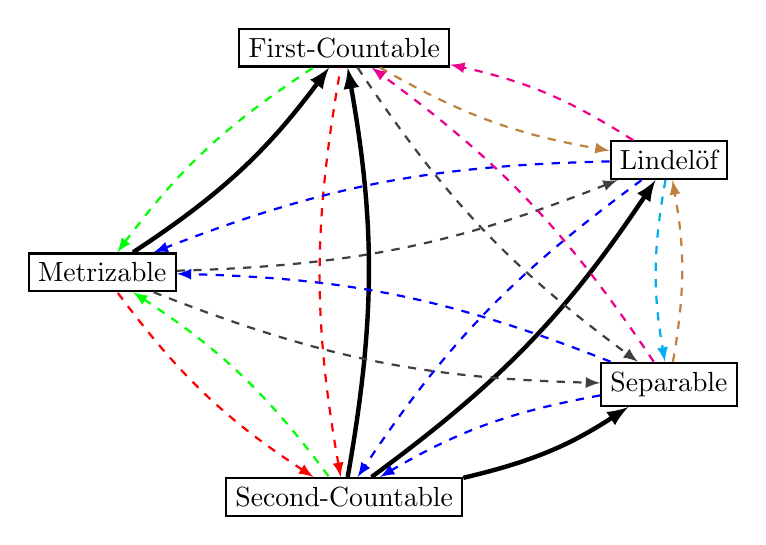
\begin{tikzpicture}[thick]
        \node[draw] (met) at (180:4) {Metrizable};
        \node[draw] (first) at (108:3) {First-Countable};
        \node[draw] (second) at (-108:3) {Second-Countable};
        \node[draw] (lind) at (24:3.5) {Lindelöf};
        \node[draw] (sep) at (-24:3.5) {Separable};

        \draw[->, >=latex, bend right=10, ultra thick] (met) edge (first);
        \draw[<-, >=latex, bend left=10, green] (met) edge[dashed] (first);
        \draw[->, >=latex, bend right=10, ultra thick] (second) edge (first);
        \draw[<-, >=latex, bend left=10, red] (second) edge[dashed] (first);
        \draw[<-, >=latex, bend left=10, green] (met) edge[dashed] (second);
        \draw[<-, >=latex, bend left=10, red] (second) edge[dashed] (met);
        \draw[->, >=latex, bend right=10, ultra thick] (second) edge (lind);
        \draw[->, >=latex, bend right=10, ultra thick] (second) edge (sep);
        \draw[->, >=latex, bend right=10, blue] (lind) edge[dashed] (met);
        \draw[->, >=latex, bend right=10, blue] (sep) edge[dashed] (met);
        \draw[->, >=latex, bend right=10, blue] (lind) edge[dashed] (second);
        \draw[->, >=latex, bend right=10, blue] (sep) edge[dashed] (second);
        \draw[->, >=latex, bend right=10, brown] (sep) edge[dashed] (lind);
        \draw[->, >=latex, bend right=10, brown] (first) edge[dashed] (lind);
        \draw[->, >=latex, bend right=10, darkgray] (met) edge[dashed] (lind);
        \draw[->, >=latex, bend right=10, darkgray] (met) edge[dashed] (sep);
        \draw[->, >=latex, bend right=10, darkgray] (first) edge[dashed] (sep);
        \draw[->, >=latex, bend right=10, magenta] (sep) edge[dashed] (first);
        \draw[->, >=latex, bend right=10, magenta] (lind) edge[dashed] (first);
        \draw[->, >=latex, bend right=10, cyan] (lind) edge[dashed] (sep);
    \end{tikzpicture}
    \end{center}
    Counterexamples:
    \begin{itemize}[nolistsep]
        \ii ({\color{green}$\dashrightarrow$}) $X = \{0, 1\}$ with $\mcal T =
            \{\varnothing, X, \{0\}\}$ is second-countable but not Hausdorff,
            thus not metrizable.
        \ii ({\color{red}$\dashrightarrow$})
            $\RR[\omega]$ with the uniform topology is metrizable but not
            second-countable. (\Cref{exmp:RUnifNot2ndCt})
        \ii ({\color{blue}$\dashrightarrow$})
            $\RR_\ell$ ($\RR$ with the lower limit topology) is
            first-countable, Lindelöf, and separable; but it is neither
            second-countable nor metrizable. (\Cref{exmp:REllCt})
        \ii ({\color{brown}$\dashrightarrow$})
            $\RR_\ell \times \RR_\ell$ is first countable and separable, but
            it is not Lindelöf. (\Cref{exmp:sorgenfrey})
        \ii ({\color{darkgray}$\dashrightarrow$})
            $\RR$ with the discrete topology is first-countable and metrizable;
            but it is not second-countable, separable, or Lindelöf.
        \ii ({\color{magenta}$\dashrightarrow$})
            $\RR$ with the finite complement topology is separable and
            Lindelöf; but it is neither first-countable nor metrizable.
        \ii ({\color{cyan}$\dashrightarrow$})
            $\RR$ with the countable complement topology is Lindelöf;
            but it is not first-countable, metrizable, or separable.
    \end{itemize}
}

\section{Separation Axioms}

\dfn{Regular and Normal Space}{
    Let $X$ be a topological space that $\{x\}$ is closed for every $x \in X$.
    In other words, $X$ is $T_1$.
    \begin{itemize}[nolistsep]
        \ii $X$ is said to be $T_2$ if it is Hausdorff.
        \ii $X$ is said to be \textit{regular}, or $T_3$, if, for each $x \in X$
            and a closed set $B$ disjoint from $x$, there exist disjoint open
            sets $U$ and $V$ such that $x \in U$ and $B \subseteq V$.
        \ii $X$ is said to be \textit{normal}, or $T_4$, if, for each pair $A$,
            $B$ of disjoint closed sets in $X$, there exist disjoint open sets
            $U$ and $V$ such that $A \subseteq U$ and $B \subseteq V$.
    \end{itemize}
}

\nt{
    \[
        T_1 \supseteq T_2 \supseteq T_3 \supseteq T_4
    \]
}

\exmp[RKisT2butNotT3]{$T_2$ Does Not Imply $T_3$}{
    The space $\RR_K$ is $T_2$ as it is finer than the standard topology.
    The set $K = \{\,1/n \mid n \in \ZZ_+\,\}$ is closed in $\RR_K$ and
    $0 \notin K$. Suppose there are disjoint open sets $U$ and $V$ such that
    $0 \in U$ and $K \subseteq V$. Let $B$ be a basis element that $0 \in B
    \subseteq U$. Then, $B = (a, b) \setminus K$ since any open interval
    containing $0$ intersects $K$. (It must be $a < 0 < b$.) Let $n \in \ZZ_+$
    such that $1/n < b$. Then, $1/n \in K \subseteq V$. Let $B'$ be a basis
    element such that $1/n \in B' \subseteq V$. Then, $B' = (c, d)$ for some
    $c < d$. Let $\max \{\,c, 1/(n+1)\,\} < z < 1/n$. Then, $z \in B \cap B'
    \subseteq U \cap V$. Hence, $\RR_K$ is not $T_3$, \#.
}

\mlemma[T34Iff]{Another Formulation}{
    Let $X$ be a $T_1$ space.
    \begin{enumerate}[nolistsep, label=(\roman*)]
        \ii $X$ is $T_3$ if and only if, for each $x \in U$ and a neighborhood
            $U$ of $x$, there exists a neighborhood $V$ of $x$ such that
            $\cl V \subseteq U$.
        \ii $X$ is $T_4$ if and only if, for each closed set $A$ and an open
            set $U$ containing $A$, there exists an open set $V$ such that
            $A \subseteq V$ and $\cl V \subseteq U$.
    \end{enumerate}
}
\pf{Proof}{
    \hfill
    \begin{enumerate}[nolistsep, label=(\roman*)]
        \ii ($\Rightarrow$)
            $B \triangleq X \setminus U$ is a closed set and $x \notin B$; there
            exist disjoint open sets $V$ and $W$ such that $x \in V$ and
            $B \subseteq W$. Then, $\cl V$ does not intersect $B$, i.e.,
            $\cl V \subseteq U$. \checkmark

            ($\Leftarrow$)
            Let $x \in X$ and $B \subseteq X$ be a closed set with $x \notin B$.
            Then, $X \setminus B$ is a neighborhood of $x$; there exists a
            neighborhood $V$ of $x$ such that $\cl V \subseteq X \setminus B$.
            Then, $V$ and $X \setminus \cl V$ are disjoint open sets that
            contain $x$ and $B$, respectively. \checkmark

        \ii ($\Rightarrow$)
            $B \triangleq X \setminus U$ is a closed set and $A \cap B =
            \varnothing$; there exist disjoint open sets $V$ and $W$ such that
            $A \subseteq V$ and $B \subseteq W$. Then, $\cl V$ does not
            intersect $B$, i.e., $\cl V \subseteq U$. \checkmark

            ($\Leftarrow$)
            Let $A, B \subseteq X$ be disjoint closed sets in $X$. Then,
            $X \setminus B$ is an open set that contains $A$; there exists an
            open set $V$ such that $A \subseteq V$ and $\cl V \subseteq X
            \setminus B$. Then, $V$ and $X \setminus \cl V$ are disjoint open
            sets that contain $A$ and $B$, respectively. \checkmark
    \end{enumerate}
}

\thm[subspSep]{}{
    Let $X$ be a topological space and $Y \subseteq X$ be a subspace of $X$.
    \begin{enumerate}[nolistsep, label=(\roman*)]
        \ii If $X$ is $T_1$, then $Y$ is $T_1$.
        \ii If $X$ is $T_2$, then $Y$ is $T_2$.
        \ii If $X$ is $T_3$, then $Y$ is $T_3$.
    \end{enumerate}
}
\pf{Proof}{
    \hfill
    \begin{enumerate}[nolistsep, label=(\roman*)]
        \ii For each $x \in Y$, $\{x\} \cap Y = \{x\}$ is closed.
        \ii Let $x, y \in Y$ with $x \neq y$.
            Then, there exist disjoint neighborhoods $U$ and $V$ of $x$ and $y$,
            respectively, in $X$. Then, $U \cap Y$ and $V \cap Y$ are disjoint
            neighborhoods of $x$ and $y$ in $Y$, respectively.
        \ii $Y$ is already $T_1$ by (i). Let $x \in Y$ and $B$ be a closed
            set in $Y$ disjoint from $x$. Then, $\cl B \cap Y = B$ by
            \Cref{th:closureSubspace}. Hence, $x \notin \cl B$; there are
            disjoint open sets $U$ and $V$ in $X$ such that $x \in U$ and $\cl
            B \subseteq V$. Then, $U \cap Y$ and $V \cap Y$ are disjoint open
            sets and $x \in U \cap Y$ and $B \subseteq V \cap Y$.
    \end{enumerate}
}

\thm[prodSep]{}{
    Let $\{X_\alpha\}_{\alpha \in J}$ be a family of topological spaces.
    Let $X \triangleq \prod_{\alpha \in J} X_\alpha$ be endowed with either
    box or product toplogy.
    \begin{enumerate}[nolistsep, label=(\roman*)]
        \ii $X$ is $T_1$ if and only if each $X_\alpha$ is $T_1$.
        \ii $X$ is $T_2$ if and only if each $X_\alpha$ is $T_2$.
        \ii $X$ is $T_3$ if and only if each $X_\alpha$ is $T_3$.
    \end{enumerate}
}
\pf{Proof}{
    Let $\vec x = (x_\alpha)_{\alpha \in J} \in X$.
    Supopse $X$ is $T_1$(, $T_2$, or $T_3$). Then, For each $\alpha_0 \in J$,
    $X_{\alpha_0}$ is homeomorphic with the subspace
    \[
        Y \triangleq \{\,\vec y \in X \mid \forall \alpha \in J \setminus \{
        \alpha_0\},\: y_\alpha = x_\alpha\,\}\text{.}
    \]
    Hence, $X_{\alpha_0}$ is $T_1$(, $T_2$, or $T_3$).
    \begin{enumerate}[nolistsep, label=(\roman*)]
        \ii ($\Leftarrow$)
            Let $\vec x = (x_\alpha)_{\alpha \in J} \in X$.
            Then, $\{\vec x\} = \bigcap_{\alpha \in J} \pi_\alpha\inv
            (\{x_\alpha\})$ is closed.

        \ii ($\Leftarrow$)
            Let $\vec x, \vec y \in X$ with $\vec x \neq \vec y$. Then, there
            exists $\alpha_0 \in J$ such that $x_{\alpha_0} \neq y_{\alpha_0}$;
            there are disjoint neighborhoods $U_{\alpha_0}$ and $V_{\alpha_0}$
            of $x_{\alpha_0}$ and $y_{\alpha_0}$ in $X_{\alpha_0}$. Then,
            If we define $U, V \subseteq X$ by $U \triangleq \prod_{\alpha \in
            J} U_\alpha$ and $V \triangleq \prod_{\alpha \in J} V_\alpha$ where
            \[
                U_\alpha \triangleq \begin{cases}
                    U_{\alpha_0} & \text{if } \alpha = \alpha_0 \\
                    X_\alpha     & \text{otherwise}
                \end{cases} \quad\text{and}\quad
                V_\alpha \triangleq \begin{cases}
                    V_{\alpha_0} & \text{if } \alpha = \alpha_0 \\
                    X_\alpha     & \text{otherwise,}
                \end{cases}
            \]
            we find that $U$ and $V$ are disjoint neighborhoods of $\vec x$ and
            $\vec y$ in $X$.

        \ii ($\Leftarrow$)
            Let $\vec x \in X$ and let $U$ be a neighborhood of $\vec x$ in $X$.
            Choose a basis element $B = \prod_{\alpha \in J} U_\alpha$ so that
            $\vec x \in B \subseteq U$. For each $\alpha \in J$, let $V_\alpha
            = X_\alpha$ if $U_\alpha = X_\alpha$. Otherwise, by
            \Cref{lem:T34Iff}, let $V_\alpha$ be a neighborhood of $x_\alpha$
            in $X$ such that $\cl{V_\alpha} \subseteq U_\alpha$. Then, $V =
            \prod_{\alpha \in J} V_\alpha$ is a neighborhood of $\vec x$ and
            $\cl V = \prod_{\alpha \in J} \cl{V_\alpha} \subseteq B \subseteq
            U$. By \Cref{lem:T34Iff}, $X$ is $T_3$.
   \end{enumerate}
}

\exmp[RlIsT4]{$\RR_\ell$ Is $T_4$}{
    $\RR_\ell$ is $T_1$ as it is finer than the standard topology. Suppose
    $A$ and $B$ are disjoint closed sets in $\RR_\ell$. For each $a \in A$
    choose a basis element $[a, x_a)$ not intersecting $B$. This is possible
    since $\RR \setminus B$ is open in $\RR_\ell$. Similarly, for each $b \in
    B$, choose a basis element $[b, x_b)$ not intersecting $A$. Then,
    \[
        U \triangleq \bigcup_{a \in A} [a, x_a) \quad\text{and}\quad
        V \triangleq \bigcup_{b \in B} [b, x_b)
    \]
    are disjoint open sets such that $A \subseteq U$ and $B \subseteq V$.
}

\exmp[RlsrIsNotT4]{$\RR_\ell^2$ is not $T_4$}{
    The space $\RR_\ell$ is $T_3$; hence $\RR_\ell^2$ is $T_3$ by
    \Cref{th:prodSep}.

    Suppose $\RR_\ell^2$ is normal for the sake of contradiction. Let $L$ be
    a subspace of $\RR_\ell^2$ where $L \triangleq \{\,x \times (-x) \in \RR^2
    \mid x \in \RR\,\}$. Here are some facts:
    \begin{itemize}[nolistsep]
        \ii $L$ has the discrete topology. Thus, every subset of $L$ is closed
            in $L$, especially.
        \ii $L$ is closed in $\RR_\ell^2$ as it is closed in $\RR^2$, which is
            coarser than $\RR_\ell^2$.
        \ii Every subset $A$ of $L$ is closed in $\RR_\ell^2$.
        \ii For every $\varnothing \neq A \subsetneq L$, there are disjoint
            open sets $U_A$ and $V_A$ in $\RR_\ell^2$ containing $A$ and $L
            \setminus A$, respectively.
    \end{itemize}
    Here, we define a function $\theta \colon \mcal P(L) \to \mcal P(\QQ^2)$ by
    \[
        A \mapsto \begin{cases}
            \QQ^2 \cap U_A & \text{if } \varnothing \subsetneq A \subsetneq L \\
            \varnothing    & \text{if } A = \varnothing \\
            \QQ^2          & \text{if } A = L\text{.}
        \end{cases}
    \]

    To show $\theta$ is injective, let $\varnothing \subsetneq A, B \subsetneq
    L$ with $A \neq B$. \textsf{WLOG}, $A \not\subseteq B$; let $x \in A
    \setminus B$. Then, since $x \in L \setminus B$, $x \in U_A \cap V_B$.
    Since $\QQ^2$ is dense in $\RR_\ell^2$ and $U_A \cap V_B$ is open and
    nonempty, there exists $q \in \QQ^2 \cap U_A \cap V_B$. Hence,
    $\QQ^2 \cap U_A \not\subseteq \QQ^2 \cap U_B$. Therefore, $\theta$
    is injective.

    Also, the map $\psi \colon \mcal P(\ZZ_+) \to \RR$ defined by
    \[
        S \mapsto \sum_{i=1}^{\infty} \frac{a_i}{10^i}
    \] is injective where $a_i = 1$ if $i \in S$ and $a_i = 0$ if $i \notin S$.
    Thus, there exists an injective map $\psi' \colon \mcal
    P(\QQ^2) \to L$. Then, $\psi' \circ \theta$ is an injective map from
    $\mcal P(L)$ to $L$, \#. (\Cref{th:noInjSurjWithPSet})

    This shows that
    \begin{enumerate}[nolistsep, label=(\roman*)]
        \ii A product of $T_4$ spaces need not be $T_4$.
        \ii A $T_3$ space need not be $T_4$.
    \end{enumerate}
}

\nt{
    \[
        T_1 \supsetneq T_2 \supsetneq T_3 \supsetneq T_4
    \]
}
\end{document}
